\documentclass{beamer}

\usepackage{txfonts}
\usepackage{hyperref}
\usepackage{fancybox}
\usepackage{xfrac}
\usepackage{cancel}


\newcommand{\heart}{\ensuremath\heartsuit}

\usepackage{mathtools,amssymb}
\newcommand{\myarrow}{\scalebox{2}[2]{$\mathclap{\curvearrowleft}\mkern2.2mu
                                                 \mathclap{\curvearrowright}$}}

\DeclareMathOperator{\Bin}{\mathrm{Bin}}

\hypersetup{colorlinks=false,linkbordercolor=red,linkcolor=green,pdfborderstyle={/S/U/W 1}}

\addtobeamertemplate{navigation symbols}{}{ \hspace{1em}    \usebeamerfont{footline}%
    \insertframenumber / \inserttotalframenumber}

\geometry{papersize={15cm,13cm}}
\usepackage{lipsum}

\makeatletter
\newenvironment<>{contdproof}[1][\proofname]{%
    \par
    \def\insertproofname{#1\@addpunct{.}}%
    \usebeamertemplate{proof begin}#2}
  {\usebeamertemplate{proof end}}
\makeatother


\setbeamertemplate{theorems}[numbered]

\newtheorem*{nonumdefinition}{Definition}
\newtheorem*{nonumproblem}{Problem}
\newtheorem*{nonumtheorem}{Theorem}
\newtheorem*{nonumremark}{Remark}
\newtheorem*{answer}{Answer}
\newtheorem*{nonumremarks}{Remarks}
\newtheorem*{nonumexamples}{Examples}
\newtheorem*{nonumsolution}{Solution}
\newtheorem*{nonumexample}{Example}
\newtheorem*{nonumproposition}{Proposition}
\newtheorem{proposition}[theorem]{Proposition}


\theoremstyle{alphtheorem}
\newtheorem{alphtheorem}{Theorem}
\renewcommand{\thealphtheorem}{\Alph{alphtheorem}}
\renewcommand{\thesection}{\arabic{section}}



\usepackage{tikz}
\newcommand*\mycirc[1]{%
  \tikz[baseline=(C.base)]\node[draw,circle,inner sep=.7pt](C) {#1};\:
}

\newcommand\myheading[1]{%
  \par\bigskip
  {\color{blue}{\large #1}}\par\smallskip}

%\usetheme{Warsaw}
%\usetheme{Berkeley} %sample 1

\usetheme{Berlin} % sample 2
%\usetheme{AnnArbor} % sample 3

\let\otp\titlepage
\renewcommand{\titlepage}{\otp\addtocounter{framenumber}{-1}}

\title{Lecture 28 : The t-distribution(s) and the Gosset/Student Theorem}
\author{}
\date{}

\begin{document}
\begin{frame}[plain]
\titlepage
\end{frame}

\begin{frame}
The following distribution {\it and its importance} was discovered by William Gosset who published under the pseudonym ``Student''. 

\begin{nonumdefinition}
A continuous random variable $T_\nu$ is sad to have $t$-{\it distribution with $\nu$ degrees of freedom} abbreviated $T_\nu \sim t_\nu$ if its pdf $f_{T_\nu}$ is given by 
$$
f_{T_\nu} (t) = \frac{\Gamma \left( \frac{\nu+1}{2}\right)}{\sqrt{\nu \Pi} \Gamma (\nu/2)} \frac{1}{\left(1+ \frac{t^2}{\nu}\right)^{\frac{\nu+1}{2}, -\infty < t < \infty}}
$$
\end{nonumdefinition}
\end{frame}

\begin{frame}
\begin{nonumdefinition}[Cont.]
\centerline{\includegraphics{figure/art28-1(a).eps}}

The graph of $f_{T_\nu} (t)$ is like the graph of the standard normal density 
$f_{Z} (z) = \dfrac{1}{\sqrt{2\pi}} e^{-t^{2}/2}$ except it doesn't go to zero as fast of $\infty$ and $-\infty$.

In fact
\begin{equation*}
\lim\limits_{\nu \to \infty} f_{T_\nu} (t) = \frac{1}{\sqrt{2\pi}} e^{- t^2/2} \tag{$\ast$}\label{eq-*}
\end{equation*}
This is why you can get $z_{\alpha}$ from the last line $(\nu = \infty)$ on the back flop of the text.

Note that $f_{T_\nu} (t) = f_{T_\nu} (-t)$ 
\end{nonumdefinition}
\end{frame}


\begin{frame}
\begin{nonumdefinition}[Cont.]
So, if $F_{T_\nu} (t)$ is the $cdf$ of $T_\nu$ we have the functional equation
$$
F_{T_\nu} (-t) = 1 - F_{T_\nu} (t)
$$
and 
$$
F_{T_\nu} (a) - F_{T_\nu} (-a) = 2 F_{T_\nu} (a) -1
$$
Or in other words, ``the handy formula'' 
$$
P\left( -a \leq T_\nu \leq a\right) = 2 F_{T_\nu}  (a)-1 
$$
holds just as for the standard normal distribution $Z$.
\end{nonumdefinition}
\end{frame}


\begin{frame}
\myheading{Comparison between the different $t$-curves and the $Z$-curve}

\centerline{\includegraphics{figure/art28-2(a).eps}}

\begin{align*}
f_{T_1} (0) & = \frac{\Gamma (1)}{\sqrt{\pi} \Gamma (\frac{1}{2})} = \frac{1}{\sqrt{\pi} \sqrt{\pi}} = \frac{1}{\pi}\\
f_{T_3} (0) & = \frac{\Gamma (2)}{\sqrt{2\pi} \Gamma (3/2)} = \frac{1}{\sqrt{2\pi} \frac{\sqrt{\pi}}{2}} = \frac{2}{\sqrt{2} \pi}  = \frac{\sqrt{2}}{\pi}\\
f_{T_5} (0) & = \frac{\Gamma (3)}{\sqrt{3\pi} \Gamma \left(\frac{J}{2} \right)} = \frac{2}{\sqrt{3\pi} (\frac{3}{2}) (\frac{1}{2}) \sqrt{\pi}} = \frac{8}{3\sqrt{3} \pi}
\end{align*}
\end{frame}

\begin{frame}
\myheading{The Critical Values of $T_\nu$}

\begin{definition}
Let $\alpha$ be a real number between $0$ and 1. Then the $\alpha$-th critical value $t_{\alpha,\nu}$ for $T_\nu$ is the number satisfying
$$
P(T_\nu \geq t_{\alpha, \nu})  = \alpha
$$
Geometrically we have
\centerline{\includegraphics{figure/art28-3(a).eps}}

So the area under the graph of $f_{T_\nu}$ to the right of the vertical line $t = t_{\alpha, \nu}$ is $\alpha$.
\end{definition}
\end{frame}

\begin{frame}
The critical values $t_{\alpha}, \nu$ are on the back flop of the text
\begin{center}
\textbf{Table A.5 Critical Values for $t$ Distributions}
\end{center}
\begin{center}
{\renewcommand{\arraystretch}{0.9}
\begin{tabular}{ccccc}
\hline
v $\backslash$ & .10 & .05 & .025 & .01\\
\hline
1 & 3.078 & 6.314 & 12.706 & \\
2 & 1.886 & 2.920 & 4.303 &\\
3 & 1.638 & 2.353 & 3.182 &\\
4 & 1.533 & 2.132 & 2.776 &\\
5 & 1.476 & 2.015 & 2.571 &\\
6 & 1.440 & 1.943 & 2.447 &\\
7 & 1.415 & 1.895 & 2.365 &\\
8 & 1.397 & 1.860 & 2.306 &\\
9 & 1.383 & 1.833 & 2.262 &\\
10 & 1.372 & 1.812 & 2.228 &\\
11 & 1.363 & 1.796 & 2.201 &\\
12 & 1.356 & 1.782 & 2.179 &\\
13 & 1.350 & 1.771 & 2.160 &\\
14 & 1.345 & 1.761 & 2.145 &\\
15 & 1.341 & 1.753 & 2.131 &\\
16 & 1.337 & 1.746 & 2.120 &\\
17 & 1.333 & 1.740 & 2.110 &\\
18 & 1.330 & 1.734 & 2.101 &\\
19 & 1.328 & 1.729 & 2.093 &\\
\hline
\end{tabular}}
\end{center}

$t_{9.05} = 1.833$ 
\end{frame}

\begin{frame}
Why is the $t$-distribution important?

Gosset/Students great observation was (probably Fisher proved this-see the Wikipedia article)

\begin{theorem}[F6]
Suppose $Z \sim N (0, 1)$ and $V \sim \chi^2 (m)$ and $Z$ and $V$ are independent. Put
$$
T = \frac{Z}{\sqrt{V/m}}
$$
Then $T \sim t_m$
\end{theorem}

\begin{nonumremark}
Of course the main point was to realize that one should look at the above ratio. In fact it seems Gosset left out the $\sqrt{m}$-from Wikipedia.
\end{nonumremark}
\end{frame}

\begin{frame}
\begin{nonumremark}
Now we do we want to look at the above ratio?
What was Gosset's idea?
Well, in the formula for the $Z$-confidence interval we were led to
$$
Z = \frac{\overline{X} - \mu }{\sigma/ \sqrt{n}}
$$
But what if {\it we don't know $\sigma$. Idea}

Replace $\sigma$ by its point estimator $S$ so we replace
$$
\frac{\overline{X} - \mu }{\sigma/\sqrt{n}} \text{~~ by ~~} \frac{\overline{X}-\mu}{S/\sqrt{n}}
$$
\end{nonumremark}
\end{frame}

\begin{frame}
From Theorem $FG$ (which is moderately hard to prove) it is on exercise in fractions to prove

\begin{alphtheorem}
Suppose $X_1, X_2, \ldots, X_n$ is a random sample from a normal population with mean $\mu$ and variance  $\sigma^2$. Then
\begin{equation*}
T = \frac{\overline{X} - \mu}{S/\sqrt{n}} \sim t_{n-1} \tag{$\ast\ast$}\label{eq-**}
\end{equation*}
We will need the results from $page$ 5 of Lecture 25
\begin{itemize}
\item[(i)] $\overline{X} \sim N \left(\mu, \dfrac{\sigma^2}{n} \right)$
\item[(ii)] $\dfrac{n-1}{\sigma^2} S^2 \sim \chi^2 (n-1)$
\item[(iii)] $\overline{X}$ and $S^2$ are independent
\end{itemize}
\end{alphtheorem}
\end{frame}

\begin{frame}
\setcounter{alphtheorem}{0}
\begin{alphtheorem}[Cont.]
Now we will prove \eqref{eq-**}.

The idea is we want to change $\overline{X}-\mu$ into $Z$ so we have to divide the numerator by $\sigma/\sqrt{n}-$ so we also have to divide the denominator by $\dfrac{\sigma}{\sqrt{n}}$ so that the fraction has the same value
\begin{align*}
\frac{\overline{X} - \mu}{(S/\sqrt{n})} & = \frac{(\overline{X} -\mu) / (\sigma/\sqrt{n})}{(S/\sqrt{n})/(\frac{\sigma}{\sqrt{n}})} = \frac{Z}{\left(\frac{\frac{S}{\cancel{\sqrt{n}}}}{\frac{\sigma}{\cancel{\sqrt{n}}}} \right)}\\
& = \frac{Z}{\left(\frac{S}{\sigma} \right)} = \frac{Z}{ \sqrt{\frac{S^2}{\sigma^2}}}\\
N & = \frac{Z}{\sqrt{\frac{n-1}{\sigma^2} S^2 \frac{1}{n-1}}}
\end{align*}
\end{alphtheorem}
\end{frame}

\begin{frame}
\setcounter{alphtheorem}{0}
\begin{alphtheorem}[Cont.]
Put $V = \dfrac{n-1}{\sigma^2} S^2$ so $V \sim \chi^2 (n-1)$.

Hence we obtain
$$
\frac{\overline{X} - \mu}{(S/\sqrt{n})} = \frac{Z}{\sqrt{V/n-1}}
$$
But by this is exact the right ratio to get a $t$-distribution with $n-1$ degrees of freedom.
\end{alphtheorem}

\begin{nonumremark}
Before Gosset statisticians  assumed that $\dfrac{\overline{X} - \mu}{S/\sqrt{n}}$ was standard normal.
This is approximately true if $n$ is large but for from true if $n$ is not large.
\end{nonumremark}
\end{frame}

\begin{frame}
\myheading{William Sealy Gosset}

From Wikipedia, the free encyclopedia

\begin{minipage}[c]{7cm}
\medskip
\textbf{William Sealy Gosset} (June 13, 1876-October 16, 1937) is famous
as a statistician, best known by his pen name \textbf{\textit{Student}} and for his
work on Student's t-distribution.

\medskip
Born in Canterbury, England to Agnes Sealy Vidal and Colonel
Frederic Gosset, Gosset attended Winchester College before reading
chemistry and mathematics at New College, Oxford. On graduating in
1899, he joined the Dublin brewery of Arthu Guinness \& Son.
\end{minipage}
\quad
\begin{minipage}[c]{5cm}
\begin{tabular}{|c|}
\hline
\textbf{William Sealy Gosset}\\
\includegraphics{figure/William_Sealy_Gosset4.eps}\\
{\tiny{\textit{Student} in 1908}}\\
\begin{tabular}{rl}
{\tiny\textbf{Born}} & {\tiny June 13, 1876}\\[-0.2cm]
& {\tiny Canterbury, Kent, England}\\
{\tiny\textbf{Died}} & {\tiny October 16, 1937 (aged 61)}\\[-0.2cm]
& {\tiny Beaconsfield, Buckinghamshire, England}
\end{tabular}\\
\hline
\end{tabular}
\end{minipage}
\end{frame}

\begin{frame}
Guinness was a progressive agro-chemical business and Gosset would
apply his statistical knowledge both in the brewery and on the
farm-to the selection of the best yielding varieties of barley. Gosset
acquired that knowledge by study, trial and error and by spending two
terms in 1906-7 in the biometric laboratory of Karl Pearson. Gosset
and Pearson had a good relationship and Pearson helped Gosset with
the mathematics of his papers. Pearson helped with the 1908 papers
but he had little appreciation of their importance. The papers
addressed the brewer's concern with small samples, while the
biometrician typically had hundreds of observations and saw no
urgency in developing small-sample methods.

Another researcher at Guinness had previously published a paper containing trade secrets of the Guinness brewery. To prevent further disclosure of confidential information, Guinness prohibited its employees from publishing any papers regardless of the contained information. This meant that Gosset was unable to publish his works under his own name. He therefore used the pseudonym \textit{Student} for his publications to avoid their detection by his employer. Thus his most famous achievement is now referred to as Student's t-distribution, which might otherwise have been Gosset's t-distribution.
\end{frame}

\begin{frame}
Gosset had almost all of his papers including \textit{The probable error of a mean} published in Pearson's journal \textit{Biometrika} using the pseudonym \textit{Student}. However, it was R. A. Fisher who appreciated the importance of Gosset's small-sample work, after Gosset had written to him to say \textit{I am sending you a copy of Student's Tables as you are the only man that's ever likely to use them!}. Fisher believed that Gosset had effected a ``logical revolution". Ironically the $t$-statistic for which Gosset is famous was actually Fisher's creation. Gosset's statistic was $z = t/\surd (n-1)$. Fisher introduced the $t$-form because it fit in with his theory of degrees of freedom. Fisher was also responsible for the applications of the $t$-distribution to regression.

Although introduced by others, Studentized residuals are named in Student's honor because, like the problem that led to Student's $t$-distribution, the idea of adjusting for estimated standard deviations is central to that concept.

Gosset's interest in barley cultivation led him to speculate that design of experiments should aim, not only at improving the average yield, but also at breeding varieties whose yield was insensitive (robust) to variation in soil and climate. This principle only occurs in the later thought of Fisher and then in the work of Genichi Taguchi in the 1950s.

In 1935, he left Dublin to take up the position of Head Brewer, in charge of the scientific side of production, at a new Guinness brewery at Park
 Royal in North West London. He died in Beaconsfield, England of a heart attack.
\end{frame}

\begin{frame}
Gosset was a friend of both Pearson and Fisher, an achievement, {\it for each had a massive ego and a loathing for the other}.$^{[\textit{citation neede I should say so!!}]}$ Gosset was a modest man who cut short an admirer with the comment that ``Fisher would have discovered it all anyway''
\end{frame}

\begin{frame}[allowframebreaks]
        \frametitle{Bibliography}
        \bibliographystyle{plain}
\begin{itemize}
\item \textit{The application of the law of error to the work of the Brewery} (1904, nota interna presso \textit{Guinness})

\item ``On the error of counting with hremacytometer''. \textit{Biometrika} \textbf{5} (3): 351-360. February 1907.

\item ``The probable error of a mean'' (\url{http://www.york.ac.uk/depts/maths/histstat/student.pdf}). \textit{Biometrika} {\bf 6} (1): 1-25. March 1908. doi:10.1093/biomet/6.1.1 (\url{http://dx.doi.org/10.1093\%2Fbiomet\%2F6.1.1}). \url{http://www.york.ac.uk/depts/maths/histstat/student.pdf}.

\item ``Probable error of a correlation coefficient''. \textit{Biometrika} \textbf{6} (2/3): 302-310. September 1908. doi:10.1093/biomet/6.2-3.302 (http://dx.doi.org/1O.1093\%2Fbiomet\%2F6.2-3.302).

\item ``The distribution of the means of samples which are not drawn at random''. \textit{Biometrika} {\bf 7} (1/2): 210-214· July-October 1909. doi:10.1093/biomet/7.1-2.210 (\url{http://dx.doi.org/10.1093\%2Fbiomet\%2F7.1-2.210}).

\item ``An experimental determination of the probable error of Dr Spearman's correlation coefficients''. \textit{Biometrika} \textbf{13} (2/3): 263-282. July 1921. doi:1O.l093/biomet/13.2-3.263 (\url{http://dx.doi.org/10.1093\%2Fbiomet\%2F13.2-3.263)}.

\item ``Review of Statistical Methods for Research Workers (R. A. Fisher)'' (\url{http://www.economics.soton.ac.uk/staff/aldrich/fisherguide/student.htm}). \textit{Eugenics Review} \textbf{18}: 148-150. 1926. \url{http://www.economics.soton.ac.uk/staff/aldrich/fisherguide/student.htm}.

\item ``On Student's 1908 Article ``The Probable Error of a Mean''(S.L.Zabell)'' (\url{http://cda.mrs.umn.edu/$\sim$jongmink/Stat2611/s1.pdf}). \textit{Journal of the American Statistical Association} \textbf{Vol. 103, No. 481:} 1-7. March 2008. \url{http://cda.mrs.umn.edu/~jongmink/Stat2611/s1.pdf}.

\item \textit{`Student's' Collected Papers} (edited by E.S. Pearson and John Wishart, with a foreword by Launce McMullen), London: Biometrika Office. (1942)
\end{itemize}
\end{frame}

\begin{frame}
\myheading{Biographies}
\begin{itemize}
\item E. S. Pearson (1990) `\textit{Student', A Statistical Biography of William Sealy Gosset}, Edited and Augmented by R.
L. Plackett with the Assistance of G. A. Barnard, Oxford: University Press.

\item E. S. Pearson, `\textit{Student}' as Statistician, \textit{Biometrika} Vol. 30, No. 3/4 (Jan., 1939), pp. 210-250.
\end{itemize}
\end{frame}

\begin{frame}
\myheading{External links}
\begin{itemize}
\item Biography by Heinz Kohler (\url{http://www.swlearning.com/quant/kohler/stat/biographical_sketches/bio12.1.html})

\item Tales of Statisticians by E. Bruce Brooks (\url{http://www.umass.edu/wsp/statistics/tales/gosset.html})

\item Student's T Distribution (\url{http://www-stat.stanford.edu/~naras/jsm/TDensity/TDensity.html})

\item Earliest known uses of some of the words of mathematics: S (\url{http://jeff560.tripod.com/s.html}) under the heading of ``Student's $t$-distribution'', describes briefly how Student's $z$ became $t$.

\item O'Connor, John J.; Robertson, Edmund F., ``William Sealy Gosset'' (\url{http://www-history.mcs.st-andrews.ac.uk/Biographies/Gosset.html}), \textit{MacTutor History of Mathematics archive}, University of St Andrews, \url{http://www-history.mcs.st-andrews.ac.uk/Biographies/Gosset.html}.
\end{itemize}
\end{frame}

\begin{frame}
Retrieved from ``\url{http://en.wikipedia.org/wiki/William_Sealy_Gosset''} Categories: 1876 births | 1937 deaths | People from Canterbury | Old Wykehamists | Alumni of New College, Oxford  | British mathematicians | Deaths from myocardial infarction | English statisticians

\rule{\textwidth}{0.03cm}

\begin{itemize}
\item This page was last modified on 1 February 2010 at 23:41. 

\item Text is available under the Creative Commons Attribution-ShareAlike License; additional terms may apply. See Terms of Use for details.

Wikipedia\textregistered\ is a registered trademark of the Wikimedia Foundation, Inc., a non-profit organization.
\end{itemize}
\end{frame}
\end{document}

